\thispagestyle{empty}
\begin{center}
%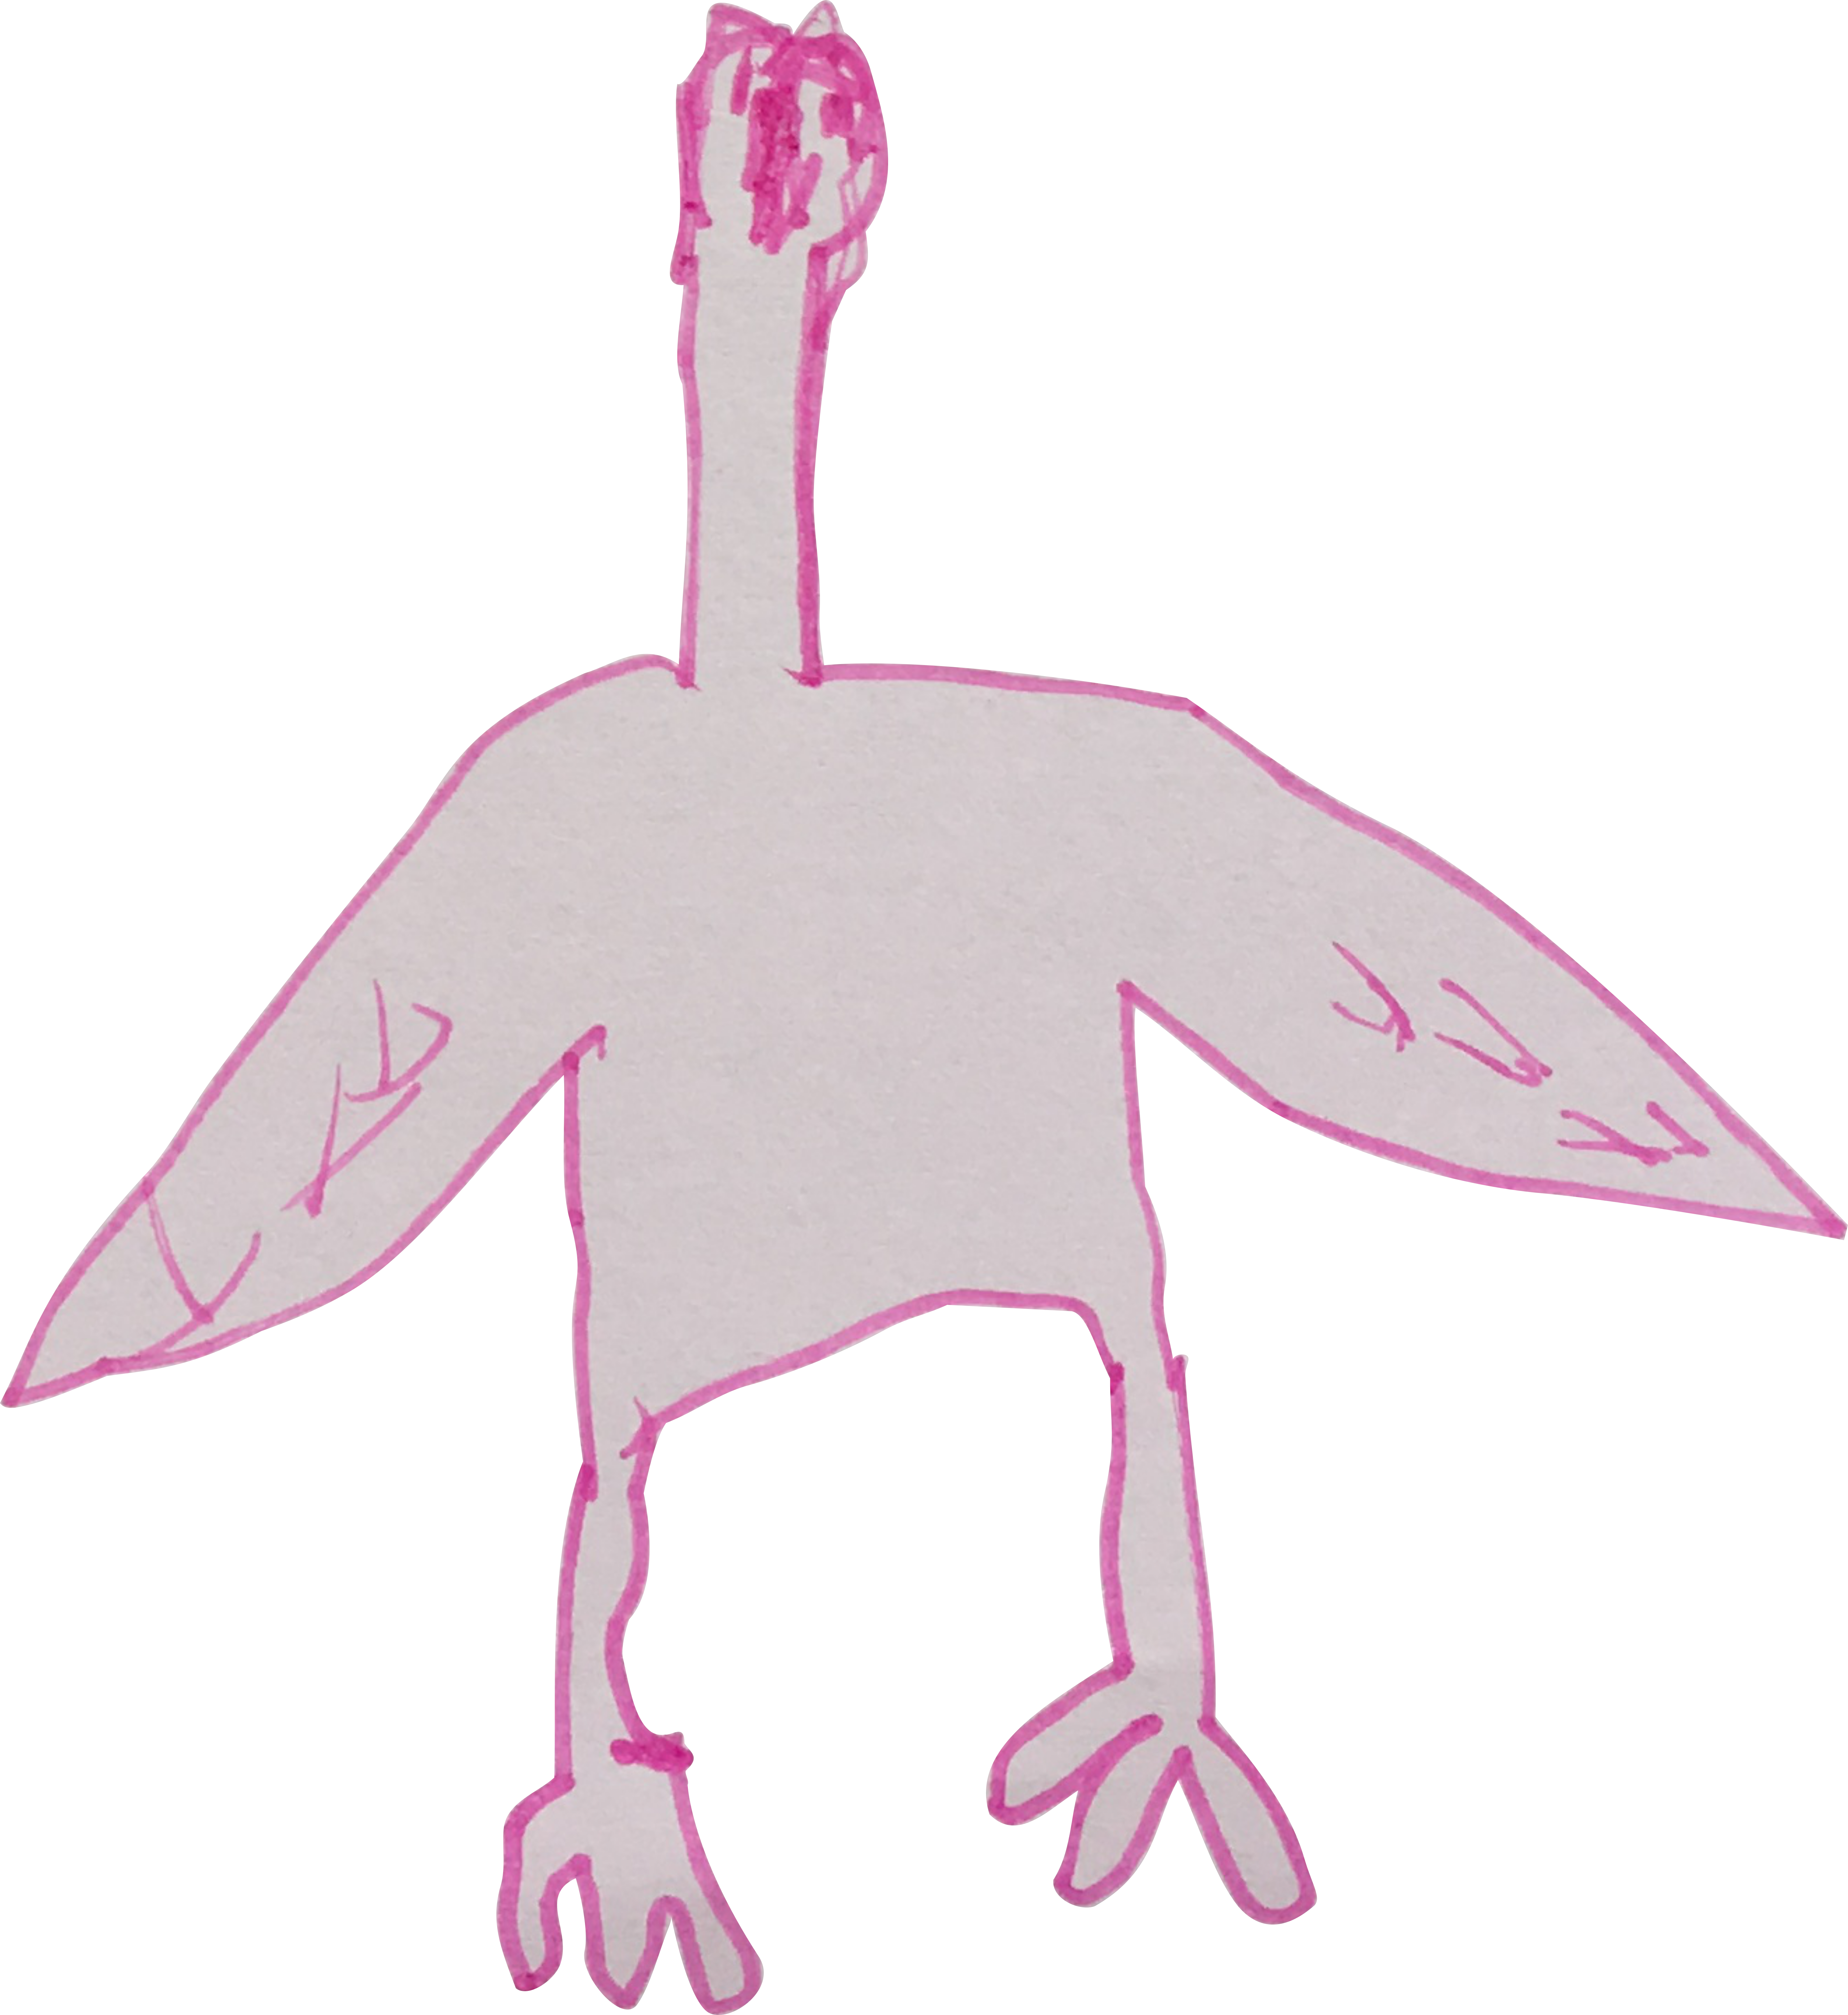
\includegraphics[height=.7\textheight]{./bilder/huhn2.png}
\end{center}
\vskip 2cm
{\Huge\color{farbe}\hfill{\tt{Prinzessin Lea}}}
\addcontentsline{toc}{chapter}{Prinzessin Lea}
\newpage
%%%%%%%%%%%%%%%%%%%%%%%%%%%%%%%%%%%%%%%%%%%%%%%%%%%%%%%%%%%%%%%%%%%%%%%%%%%%%%%
\lettrine[lines=2, lhang=.2, loversize=.25, lraise=0.05, findent=0.1em,
nindent=0em]{{\textooquote}I}{n} jeder Stadt gibt es einen Zauberer oder eine Hexe, die dafür sorgen müssen, dass die vielen magischen Wesen nicht zu viel Unsinn treiben und die Menschen möglichst in Ruhe lassen. Von diesen magischen Wesen gibt es übrigens viel mehr als man denkt, sie sind nur meistens unsichtbar und halten sich aus der echten Welt heraus. Eigentlich gibt es sogar alle magischen Wesen, von denen man je gehört hat. Vampire, Gespenster, Feen, Einhörner und noch viele andere, die oft nicht mal einen Namen haben. Aber fast alle haben zugestimmt, dass sie uns Menschen nur in Geschichten besuchen und uns sonst in Ruhe lassen. 

Aber manchmal kommen sie eben doch zu uns und dafür gibt es uns. Bei uns in der Stadt bin ich die Hexe. Das entscheidet sich ganz kurz vor der Geburt. Wenn ein Zauberer oder eine Hexe stirbt, wird das nächste Kind, das geboren wird der Nachfolger. Und bei uns hat es eben mich getroffen. Das ist viel blöder, als man vielleicht denkt.

Da sind zum Beispiel doe Regeln, an die man sich halten muss. Ich darf nichts einfach nur für mich hexen. Wenn ich vergessen habe, die Hausaufgaben zu machen, darf ich nicht einfach einen Zauberspruch verwenden, ich muss die selbst machen. Und wenn kein Apfelsaft mehr im Kühlschrank ist, muss ich genauso in den Supermarkt wie jeder andere auch, obwohl es leicht wäre, die ganze Wohnung in einen Swimmingpool aus Orangensaft zu verwandeln. Denn jeder Zauberspruch öffnet ein Loch in die magsiche Welt und einige Wesen warten nur darauf, in unsere Welt geschlüpft zu kommen. Erst neulich hat ein Schattenbär beinahe ein Haus zum Einsturz gebracht, weil er in der Küche Honig gewittert hat. 


